\documentclass[border=7pt]{standalone}
\usepackage{tkz-euclide}
\usetkzobj{all} % on charge tous les objets

\begin{document}
  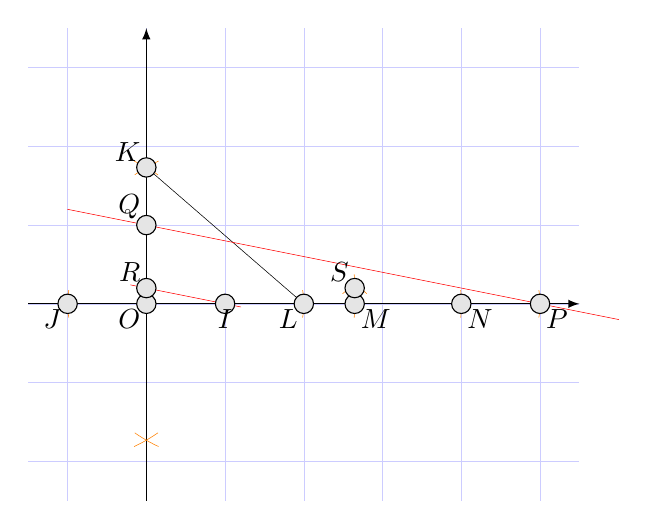
\begin{tikzpicture}[inner sep=2pt]
    % grille et axes
    \draw[very thin,color=blue!20] (-1.5,-2.5) grid (5.5,3.5);
    \draw (-1.5,0) edge[-latex] (5.5,0) (0,-2.5) edge[-latex] (0,3.5);
    % définition des points
    \pgfmathsetmacro\sqt{sqrt(3)}
    \pgfmathsetmacro\sqs{sqrt(7)}
    \tkzDefPoints{0/0/O, 1/0/I,-1/0/J, 0/\sqt/K, 0/-\sqt/-K, 2/0/L, \sqs/0/M, 4/0/N, 5/0/P, 0/1/Q, 0/0.2/R, \sqs/0.2/S}
    % compas
    \tkzCompasss[color = orange,length = .35](I,K J,K I,-K J,-K O,J I,L O,M L,N N,P M,S R,S)
    % lignes et segments
    \tkzDrawSegments(K,L)
    \tkzDrawLine[very thin,color=red](P,Q)
    \tkzDrawLine[very thin,color=red](I,R)
    % points
    \tkzDrawPoints[size=7](O,I,J,K,L,M,N,P,Q,R,S)
    \tkzLabelPoints[below](I)
    \tkzLabelPoints[below left](O,J,L)
    \tkzLabelPoints[below right](M,N,P)
    \tkzLabelPoints[above left](K,Q,R,S)
  \end{tikzpicture}
\end{document}
